\section{The Text-Carbon Dataset: Construction and Characteristics} % 更改标题以更突出数据集本身
\label{sec:Data}

Addressing the critical need for nuanced, event-aware carbon emission analyses, this paper proposes the Text-Carbon Dataset which uniquely integrates high-frequency daily carbon emission time series with contemporaneous, AI-verified textual narratives of socio-economic, policy, and environmental events. The raw temporal data comprise daily carbon emission estimates for 20 distinct administrative regions across China, spanning the period from January 1, 2019, to December 31, 2024. The dataset offers sectoral disaggregation where feasible, covering key emitting sectors such as industry, power generation, ground transportation, aviation, and residential consumption. Before processing, we conducted outlier handling and ultimately retained multi-domain carbon emission data from 13 provinces without outliers.


This section first outlines the foundational data sources and the geographical and sectoral scope of the dataset. It then elaborates on the two-stage methodology developed for its construction (as in Figure \ref{fig:dataprocess}): (1) an advanced change-point detection and characterization phase to pinpoint significant emission shifts, and (2) an AI-driven information retrieval phase to collect and align pertinent event texts. Finally, we describe the key characteristics of the resulting dataset and its public availability.

\begin{figure*}[ht]
    \centering
    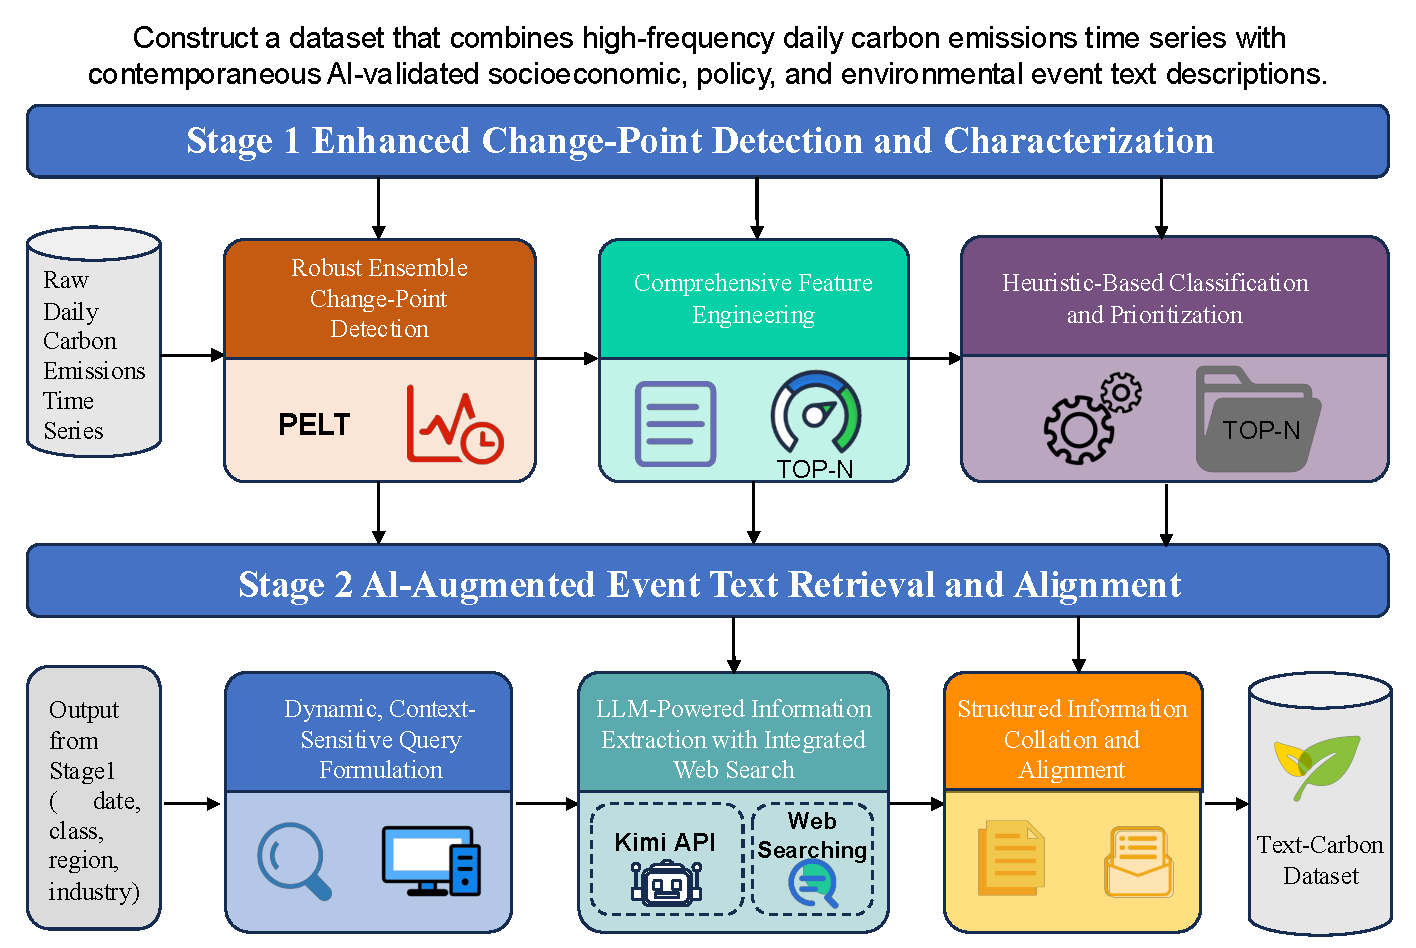
\includegraphics[width=0.8\textwidth]{Figure/data_process.pdf}
    \caption{data}
    \label{fig:dataprocess}
\end{figure*}



\subsection{Systematic Multi-Stage Dataset Construction Methodology}
\label{subsec:DatasetMethodology}
The Text-Carbon Dataset was synthesized via a systematic, largely automated, two-stage pipeline. This pipeline was engineered to first discern statistically significant and potentially anomalous junctures within the emission time series, and subsequently to enrich these junctures with contextually pertinent event-specific textual information. The entire methodology is implemented through a suite of custom Python scripts, which are made available with the dataset, facilitating reproducibility and further development by the research community.


\subsubsection{Stage 1: Enhanced Change-Point Detection and Characterization}
\label{subsubsec:ChangePointEnhancement}
The foundational stage involved the rigorous identification and in-depth characterization of significant change-points within each daily carbon emission time series. The objective was to isolate moments of substantial deviation from established patterns, particularly those not attributable to simple periodicity, thereby flagging them as candidates for event-driven analysis. The procedure encompassed several critical steps:
\begin{itemize}
\item \textbf{Robust Ensemble Change-Point Detection:} To ensure comprehensive capture of diverse discontinuity types, an ensemble of change-point detection algorithms was employed. This primarily utilized the computationally efficient Pelt algorithm renowned for its precision in multiple change-point scenarios. This was synergistically supplemented by algorithms for local extreme value identification (pinpointing sharp deviations from localized statistical norms) and the analysis of high-magnitude first-order differences (indicative of abrupt value shifts). This integrated methodology, implemented within our data processing pipeline, provided a robust set of candidate change-points.
\item \textbf{Comprehensive Feature Engineering:} Each candidate change-point underwent extensive feature extraction through a dedicated analytical module. A rich set of over a dozen statistical and morphological features was computed for temporal windows preceding and succeeding each point. These features quantified diverse aspects, including the absolute and relative magnitudes of the change, alterations in local trend (slope) and volatility (variance), measures of time series stability, and crucially, several metrics designed to assess the degree of seasonality and periodicity (ACF-derived periodicity strength, lagged correlations for annual and monthly cycles). A primary aim of this feature engineering was to differentiate change-points exhibiting strong non-periodic characteristics from those merely reflecting regular cyclical variations.
\item \textbf{Heuristic-Based Classification and Prioritization:} Leveraging this comprehensive feature set, a heuristic-driven, rule-based classification model assigned each change-point to one of several predefined categories ('Policy-induced', 'Discrete Event', 'Seasonal Shift', 'Trend Alteration'), accompanied by a numerically derived confidence score. The classification rules were informed by domain knowledge, with weights specifically designed to elevate the significance of non-periodic features for 'Policy-induced' and 'Discrete Event' categories. Subsequently, a prioritization filter selected the top-10 most confident and distinct change-points per time series for the subsequent information retrieval stage, ensuring a focused and resource-efficient approach.
\end{itemize}
This stage culminated in a structured, machine-readable list of highly characterized and classified change-points for each regional and sectoral emission series, thereby providing a targeted input for the subsequent event contextualization phase.


\subsubsection{Stage 2: AI-Augmented Event Text Retrieval and Alignment}
\label{subsubsec:EventTextRetrieval}
Following the identification of prioritized change-points, the second stage focused on the automated retrieval and precise alignment of relevant textual narratives describing policies or events. This was orchestrated by a dedicated information retrieval module, which strategically employed a Large Language Model (LLM)—specifically, Kimi, accessed via the Moonshot AI API—for nuanced information extraction:
\begin{itemize}
\item \textbf{Dynamic, Context-Sensitive Query Formulation:} For each selected change-point, a highly specific, structured query was algorithmically generated. These queries were meticulously tailored, incorporating the change-point's date, its pre-assigned classification (e.g., 'Policy-induced', 'Discrete Event'), the specific geographical region, and the relevant industrial sector. The queries directed the LLM to search for concrete policy implementations or distinct real-world occurrences within a defined temporal window bracketing the change-point. Emphasis was placed on retrieving verifiable details, such as official policy titles, issuing authorities, promulgation or effective dates, comprehensive event descriptions, and, critically, URLs to verifiable source documentation.
    \item \textbf{LLM-Powered Information Extraction with Integrated Web Search:} The formulated queries were submitted to the Kimi LLM. The interaction was governed by an elaborate system prompt, explicitly instructing the LLM to prioritize information with a direct bearing on carbon emissions, to stringently cite official or verifiable sources, and to structure its output coherently. The LLM's native web search capability (referred to as the `web\_search` tool by the API provider) was programmatically invoked, enabling it to access and synthesize information extending beyond its static pre-training corpus. To ensure operational robustness and manage API constraints, the system incorporated comprehensive error handling, API call retry mechanisms with exponential backoff, and programmed inter-call latencies.
    \item \textbf{Structured Information Collation and Temporal Alignment:} Textual information retrieved by the LLM was systematically parsed and temporally aligned with the corresponding change-point. The definitive output for each processed carbon emission series was a structured text file containing the event narratives. These files, formatted for straightforward ingestion by our custom data loading utilities, catalogue each significant change-point by date and classified type, followed by the detailed textual narrative (policy specifics, event attributes) furnished by the LLM. Efficient local caching of LLM responses was implemented to obviate redundant API transactions during potential reprocessing or iterative refinement.
\end{itemize}


\subsection{Resultant Dataset Characteristics and Open Accessibility} 
\label{subsec:DatasetChar}
The Text-Carbon Dataset, an outcome of the aforementioned methodology, represents a unique resource for empirical investigations into event-driven carbon emission dynamics. Its salient characteristics include:
\begin{itemize}
\item \textbf{Spatiotemporal Coverage and Granularity:} The dataset encompasses daily carbon emission figures and precisely aligned event/policy textual narratives for 13 administrative regions within China, covering five major distinct emitting sectors, for the period January 1, 2019, to December 31, 2024.
\item \textbf{Data Volume and Richness:} It comprises thousands of observation points for the carbon emission time series. Across these series, hundreds of unique change-points have been identified, characterized, and enriched with detailed textual event/policy descriptors.
\item \textbf{Depth of Event Descriptors:} For each prioritized change-point, the dataset provides comprehensive textual narratives, including "official policy titles, promulgation dates, specific event timelines and locations, and verifiable source URLs when available"].
\item \textbf{Novelty and Contribution:} To the best of our knowledge, the Text-Carbon Dataset is among the first large-scale, publicly accessible resources to systematically integrate daily, sector-specific carbon emission data with AI-corroborated, contextually targeted event and policy textual information at this level of regional granularity for China.
\end{itemize}

While the Text-Carbon Dataset offers considerable utility, certain inherent caveats warrant consideration. The automated event retrieval, although guided by sophisticated LLM interactions and verification prompts, remains susceptible to potential omissions or inaccuracies characteristic of current LLM technologies; not all pertinent events may be captured, and the veracity of retrieved details is contingent upon the LLM's interpretation and the underlying web sources. The present geographical scope is confined to selected regions within China, and the spectrum of identified event types is predominantly those discernible through public web-accessible announcements and official documentation.